%% ============================================================
%% CoProof — Presentación de Proyecto II  (v3 — Story Arc)
%% 14 diapositivas · transición automática 15 s
%% Compilar: pdflatex coproof_presentacion.tex (2 pasadas)
%% ============================================================
\documentclass[aspectratio=169, 10pt]{beamer}

\usepackage[utf8]{inputenc}
\usepackage[T1]{fontenc}
\usepackage[spanish]{babel}
\usepackage{lmodern}
\usepackage{booktabs}
\usepackage{tikz}
\usetikzlibrary{positioning, arrows.meta, shapes.geometric, calc}
\usepackage{pgfplots}
\pgfplotsset{compat=1.18}
\usepackage{xcolor}
\usepackage{listings}
\usepackage{graphicx}
\usepackage{hyperref}
\hypersetup{pdfpagemode=FullScreen, pdfstartview=FitH, pdffitwindow=true}

\definecolor{cpBlue}{RGB}{13, 51, 109}
\definecolor{cpTeal}{RGB}{0, 128, 115}
\definecolor{cpAccent}{RGB}{200, 80, 20}
\definecolor{cpLight}{RGB}{235, 242, 252}
\definecolor{cpGray}{RGB}{80, 80, 80}
\definecolor{leanpurple}{RGB}{100, 60, 160}

\usetheme{default}
\usecolortheme[named=cpBlue]{structure}

\setbeamercolor{frametitle}{fg=cpBlue, bg=white}
\setbeamerfont{frametitle}{series=\bfseries, size=\large}
\setbeamertemplate{frametitle}{%
  \vspace{0.4em}%
  \insertframetitle\par%
  \vspace{0.15em}{\color{cpBlue!40}\hrule height 0.8pt}\vspace{0.2em}%
}

\setbeamertemplate{navigation symbols}{}
\setbeamertemplate{footline}{%
  \leavevmode%
  \hbox to \paperwidth{%
    \hfill%
    \footnotesize\color{cpGray}\insertframenumber\,/\,\inserttotalframenumber%
    \hspace{7pt}%
  }\vspace{5pt}%
}

\setbeamercolor{block title}{fg=white, bg=cpBlue}
\setbeamercolor{block body}{fg=black, bg=cpLight}
\setbeamercolor{alertblock title}{fg=white, bg=cpAccent}
\setbeamercolor{alertblock body}{fg=black, bg=cpAccent!10}
\setbeamercolor{alerted text}{fg=cpAccent}
\setbeamercolor{background canvas}{bg=white}
\setbeamercolor{normal text}{fg=black, bg=white}

\title{\textbf{CoProof}}
\subtitle{Plataforma colaborativa de demostraci\'{o}n formal de teoremas}
\author{David L\'{o}pez \and Daniel Tejeda \and Emiliano Flores}
\institute{Centro de Ense\~{n}anza T\'{e}cnica Industrial \textperiodcentered{} Proyecto Integrador II}
\date{Mayo 2026}

\newcommand{\yes}{\textcolor{cpTeal}{\checkmark}}
\newcommand{\no}{\textcolor{red}{$\times$}}

% Inline burger icon (real photo)
\newcommand{\burgericon}{%
  
\includegraphics[height=0.55cm]{img/beeschurger.jpg}%
}

\lstdefinestyle{lean}{
  language=,
  basicstyle=\ttfamily\small,
  keywordstyle=\color{leanpurple}\bfseries,
  commentstyle=\color{cpTeal}\itshape,
  morekeywords={theorem, by, induction, rw, ring, simp, have, show,
                with, zero, succ, fun, def, import, open, where},
  frame=none,
  backgroundcolor=\color{cpBlue!5},
  xleftmargin=4pt, xrightmargin=4pt,
  breaklines=true,
}

% ============================================================
\begin{document}
% ============================================================

% ── SLIDE 1 — Portada ────────────────────────────────────────
\begin{frame}
  \transduration{15}
  \vspace{0cm}
  \begin{center}
    
\includegraphics[height=5.5cm]{img/logo_bright_bg_text.pdf}\\[0.5em]
    {\color{cpGray}\large Plataforma colaborativa de demostraci\'{o}n formal de teoremas}\\[1.0em]
    \textcolor{cpBlue!40}{\rule{\textwidth}{0.6pt}}\\[0.8em]
    {\normalsize David L\'{o}pez \textperiodcentered{} Daniel Tejeda \textperiodcentered{} Emiliano Flores}\\[0.3em]
    {\small\color{cpGray} CETI --- Proyecto Integrador IDS \textperiodcentered{} Mayo 2026}
  \end{center}
\end{frame}

% ── SLIDE 2 — Atiyah ─────────────────────────────────────────
\begin{frame}{Sir Michael Atiyah y la Hip\'{o}tesis de Riemann}
  \transduration{15}
  \begin{columns}[T]
    \begin{column}{0.38\textwidth}
      \vspace{0.3cm}
      \begin{center}
        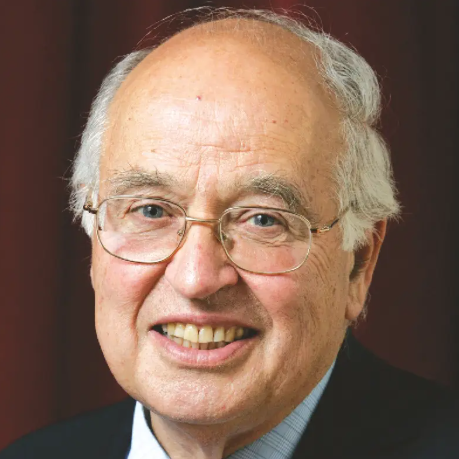
\includegraphics[width=2.6cm]{img/atiyah.png}\par\vspace{0.4em}
        {\large\color{cpBlue}\bfseries Sir Michael Atiyah}\\[0.3em]
        {\small\color{cpGray}Fields Medal 1966}\\[0.1em]
        {\small\color{cpGray}Abel Prize 2004}\\[0.5em]
        {\footnotesize\color{cpGray}Uno de los mayores\\matem\'{a}ticos del siglo XX}
      \end{center}
    \end{column}
    \begin{column}{0.58\textwidth}
      \begin{block}{Septiembre 2018}
        Anunci\'{o} una prueba de la \textbf{Hip\'{o}tesis de Riemann} ---
        uno de los 7 Problemas del Milenio, sin resolver por 160 a\~{n}os.
      \end{block}
      \vspace{0.35cm}
      \begin{itemize}
        \item La comunidad reaccion\'{o} de inmediato: discusiones, anotaciones, contra-argumentos
        \item Atiyah falleci\'{o} en \textbf{enero de 2019}
      \end{itemize}
      \vspace{0.35cm}
      \begin{alertblock}{}
        \small Meses despu\'{e}s el consenso fue claro:\\
        la prueba ten\'{i}a un \textbf{error l\'{o}gico fatal}.\\
        Llegar a ese consenso tom\'{o} \textbf{meses de colaboraci\'{o}n as\'{i}ncrona}.
      \end{alertblock}
    \end{column}
  \end{columns}
\end{frame}

% ── SLIDE 3 — El Problema ────────────────────────────────────
\begin{frame}{El Problema de Fondo}
  \transduration{15}
  \begin{columns}[T]
    \begin{column}{0.52\textwidth}
      \textbf{\textquestiondown Por qu\'{e} tard\'{o} tanto?}
      \vspace{0.3cm}
      \begin{itemize}
        \item La revisi\'{o}n de pruebas es \textbf{lenta, as\'{i}ncrona y subjetiva}
        \item No hay est\'{a}ndar verificable por m\'{a}quina para \textit{este paso es v\'{a}lido}
        \item Distribuir la revisi\'{o}n genera desacuerdos sin \'{a}rbitro neutral
        \item El consenso depende de confianza en el criterio humano
      \end{itemize}
    \end{column}
    \begin{column}{0.44\textwidth}
      \vspace{0.5cm}
      \begin{block}{\centering La pregunta clave}
        \centering\vspace{0.3cm}
        \textquestiondown Qu\'{e} pasar\'{i}a si la \textbf{correcci\'{o}n l\'{o}gica}
        fuera tan inequ\'{i}voca como un \textbf{error de compilador}?
        \vspace{0.3cm}
      \end{block}
    \end{column}
  \end{columns}
\end{frame}

% ── SLIDE 4 — Correctness ────────────────────────────────────
\begin{frame}{Correcci\'{o}n L\'{o}gica: de Matem\'{a}ticas a L\'{o}gica Pura}
  \transduration{15}
  \begin{columns}[T]
    \begin{column}{0.50\textwidth}
      \textbf{Ejemplo matem\'{a}tico}
      \vspace{0.2cm}

      \textbf{Teorema:} $\displaystyle\sum_{i=1}^{n} i = \dfrac{n(n+1)}{2}$

      \vspace{0.25cm}
      \textit{Por inducci\'{o}n:}
      \begin{itemize}\small
        \item \textbf{Base:} $n=1 \Rightarrow 1 = \frac{1\cdot2}{2}$ \yes
        \item \textbf{Paso:} si vale para $k$, vale para $k{+}1$ \yes
        \item \textbf{Conclusi\'{o}n:} vale para todo $n \geq 1$
      \end{itemize}
    \end{column}
    \begin{column}{0.46\textwidth}
      \textbf{Estructura l\'{o}gica pura}
      \vspace{0.4cm}
      \\
      \centering
      \begin{tikzpicture}[scale=0.88,
          lbox/.style={draw, rounded corners=3pt, fill=cpLight,
                       minimum width=3.8cm, minimum height=0.5cm,
                       align=center, font=\footnotesize}]
        \node[lbox] (p) at (0, 1.4) {$P$:\; propiedad en $n=1$};
        \node[lbox] (q) at (0, 0.5) {$Q$:\; prop.\ en $k \Rightarrow k{+}1$};
        \node[lbox, fill=cpTeal!20] (c) at (0,-0.5)
          {\yes\; propiedad para todo $n$};
        \draw[->, thick, color=cpBlue] (p.east) to[out=0,in=0,looseness=1.5] (c.east);
        \draw[->, thick, color=cpBlue] (q) -- (c);
        \node[font=\tiny, color=cpGray] at (0,-1.1)
          {$P,\;Q \;\vdash\; \forall n,\;\text{prop}(n)$\quad (modus ponens)};
      \end{tikzpicture}\par
      \vspace{0.15cm}
      {\small\color{cpGray}\textbf{Correcci\'{o}n} = cada paso sigue reglas admitidas.}
    \end{column}
  \end{columns}
\end{frame}

% ── SLIDE 5 — DAG + Hamburguesa ──────────────────────────────
\begin{frame}{Las Pruebas son Grafos, no Listas}
  \transduration{15}
  \begin{columns}[T]
    \begin{column}{0.43\textwidth}
      \textbf{Analog\'{i}a: preparar una hamburguesa}
      \vspace{0.4cm}\\
      \centering
      \begin{tikzpicture}[scale=0.80,
          hnode/.style={draw, rounded corners=3pt, fill=cpLight,
                        minimum width=2.2cm, minimum height=0.5cm,
                        align=center, font=\footnotesize},
          arr/.style={->, thick, color=cpBlue!60}]
        \node[hnode, fill=cpBlue!15] (asm) at (0, 0) {Ensamblar};
        \node[hnode] (bun) at (-3.0,-1.2) {Tostar pan};
        \node[hnode] (pat) at ( 0.0,-1.2) {Asar carne};
        \node[hnode] (tom) at ( 3.0,-1.2) {Picar tomate};
        \draw[arr] (asm) -- (bun);
        \draw[arr] (asm) -- (pat);
        \draw[arr] (asm) -- (tom);
        \node[font=\tiny, color=cpTeal] at (-3.0,-1.95) {independiente};
        \node[font=\tiny, color=cpTeal] at ( 0.0,-1.95) {independiente};
        \node[font=\tiny, color=cpTeal] at ( 3.0,-1.95) {independiente};
      \end{tikzpicture}\\[0.3em]
      
\includegraphics[width=2.2cm]{img/beeschurger.jpg}
    \end{column}
    \begin{column}{0.03\textwidth}\end{column}
    \begin{column}{0.50\textwidth}
      \textbf{Una prueba matem\'{a}tica funciona igual}
      \vspace{0.4cm}\\
      \centering
      \begin{tikzpicture}[scale=0.80,
          pnode/.style={draw, rounded corners=3pt,
                        minimum width=2.3cm, minimum height=0.5cm,
                        align=center, font=\footnotesize},
          arr/.style={->, thick, color=cpBlue!60}]
        \node[pnode, fill=cpBlue!15] (root) at (0, 0)    {Teorema ra\'{i}z};
        \node[pnode, fill=cpTeal!18] (la)  at (-3.0,-1.2){Lema A};
        \node[pnode, fill=cpTeal!18] (lb)  at ( 0.0,-1.2){Lema B};
        \node[pnode, fill=cpTeal!18] (lc)  at ( 3.0,-1.2){Lema C};
        \node[pnode, fill=green!22]  (ba)  at (-3.0,-2.4){\yes\ base};
        \node[pnode, fill=green!22]  (bc)  at ( 3.0,-2.4){\yes\ base};
        \node[pnode, fill=yellow!40] (bb)  at ( 0.0,-2.4){pendiente};
        \draw[arr](root)--(la);\draw[arr](root)--(lb);\draw[arr](root)--(lc);
        \draw[arr](la)--(ba);\draw[arr](lb)--(bb);\draw[arr](lc)--(bc);
      \end{tikzpicture}\par
      \vspace{0.1cm}
      {\small\color{cpGray}Lemas independientes se resuelven \textbf{en paralelo}.}
    \end{column}
  \end{columns}
\end{frame}

% ── SLIDE 6 — NL vs Lean ─────────────────────────────────────
\begin{frame}{Automatizando la Formalización con Lean 4}
  \transduration{15}
  \begin{columns}[T]
    \begin{column}{0.46\textwidth}
      \textbf{\color{cpGray}En lenguaje natural}
      \vspace{0.2cm}
      \begin{itemize}\small
        \item Un humano puede \emph{saltarse} pasos
        \item La validez depende de intuici\'{o}n compartida
        \item En colaboraci\'{o}n as\'{i}ncrona: los pasos omitidos son donde viven los desacuerdos
      \end{itemize}
      \vspace{0.3cm}
      {\footnotesize\color{cpGray}\textit{\textquotedblleft{}...y por lo tanto,
      combinando ambos lemas, se sigue el resultado.\textquotedblright{}}}
    \end{column}
    \begin{column}{0.50\textwidth}
      \textbf{\color{leanpurple}En Lean~4}
      \vspace{0.2cm}

      \colorbox{cpBlue!5}{\parbox{\linewidth}{%
        \ttfamily\footnotesize\color{leanpurple}
        theorem sum\_formula (n : Nat) :\\[1pt]
        \hspace*{0.8em}Finset.sum (Finset.range (n+1)) id\\[1pt]
        \hspace*{0.8em}= n * (n + 1) / 2 := by\\[1pt]
        \hspace*{0.4em}induction n with\\[1pt]
        \hspace*{0.4em}| zero => simp\\[1pt]
        \hspace*{0.4em}| succ k ih =>\\[1pt]
        \hspace*{1.2em}rw [Finset.sum\_range\_succ, ih]\\[1pt]
        \hspace*{1.2em}ring
      }}\par\vspace{0.25cm}
      {\small\color{cpBlue}\textbf{Si hay un error l\'{o}gico, no compila.}\\
      No hay ambig\"{u}edad. No hay debate.}
    \end{column}
  \end{columns}
\end{frame}

% ── SLIDE 7 — NL vs FL comparación ─────────────────────────
\begin{frame}{Prueba Informal vs.\ Prueba Formal}
  \transduration{15}
  \begin{columns}[T]
    \begin{column}{0.37\textwidth}
      {\color{cpGray}\bfseries\normalsize Prueba en lenguaje natural}
      \vspace{0.4cm}

      \colorbox{cpGray!10}{\parbox{\linewidth}{%
        \footnotesize
        \textbf{Teorema:} $\sqrt{2}$ es irracional.\\[0.4em]
        \itshape
        Sea $\sqrt{2} = p/q$ con $\gcd(p,q)=1$.
        Entonces $p^2 = 2q^2$, por lo que $p$ es par.
        Sea $p=2k$; entonces $q^2=2k^2$, as\'{i} $q$ es par.
        Pero $\gcd(p,q)\geq 2$. Contradicci\'{o}n.~$\square$
      }}\par\vspace{0.4cm}
      {\small\color{cpGray}\raggedright\textquestiondown Es correcta?
      Depende de que el lector acepte cada paso.}
    \end{column}
    \begin{column}{0.59\textwidth}
      {\color{leanpurple}\bfseries\normalsize Prueba en Lean~4}
      \vspace{0.4cm}

      \colorbox{cpBlue!5}{\parbox{\linewidth}{%
        \ttfamily\scriptsize\color{leanpurple}
        theorem sqrt2\_irrat :\\[1pt]
        \hspace*{0.4em}$\neg\,\exists$ (p q : $\mathbb{Z}$), q $\neq$ 0 $\wedge$\\[1pt]
        \hspace*{1.0em}Int.gcd p q = 1 $\wedge$ p\^{}2 = 2 * q\^{}2 := by\\[1pt]
        \hspace*{0.4em}intro $\langle$p, q, hq, hcop, heq$\rangle$\\[1pt]
        \hspace*{0.4em}have hp2 : 2 $\mid$ p\^{}2 :=\\[1pt]
        \hspace*{1.8em}$\langle$q\^{}2, by linarith$\rangle$\\[1pt]
        \hspace*{0.4em}have hp : 2 $\mid$ p :=\\[1pt]
        \hspace*{1.8em}Int.Prime.dvd\_of\_dvd\_pow\\[1pt]
        \hspace*{2.4em}(Int.prime\_iff.mpr (by norm\_num)) hp2\\[1pt]
        \hspace*{0.4em}obtain $\langle$k, hk$\rangle$ := hp\\[1pt]
        \hspace*{0.4em}have heq2 : (2*k)\^{}2 = 2 * q\^{}2 := by rw [\textleftarrow hk]; exact heq\\[1pt]
        \hspace*{0.4em}have hq2 : 2 $\mid$ q\^{}2 := $\langle$k\^{}2, by linarith$\rangle$\\[1pt]
        \hspace*{0.4em}have hq : 2 $\mid$ q :=\\[1pt]
        \hspace*{1.8em}Int.Prime.dvd\_of\_dvd\_pow\\[1pt]
        \hspace*{2.4em}(Int.prime\_iff.mpr (by norm\_num)) hq2\\[1pt]
        \hspace*{0.4em}have : 2 $\mid$ Int.gcd p q :=\\[1pt]
        \hspace*{1.8em}Int.dvd\_gcd hp hq\\[1pt]
        \hspace*{0.4em}rw [hcop] at this\\[1pt]
        \hspace*{0.4em}\textcolor{cpGray}{-- this : (2 : $\mathbb{Z}$) $\mid$ 1 $\Rightarrow$ $\bot$}\\[1pt]
        \hspace*{0.4em}exact absurd this (by norm\_num)
      }}
    \end{column}
  \end{columns}
\end{frame}

% ── SLIDE 8 — Lean: corrección sí, colaboración no ───────────
\begin{frame}{Lean~4: Correcci\'{o}n S\'{i},\ Colaboraci\'{o}n No}
  \transduration{15}
  \begin{columns}[T]
    \begin{column}{0.48\textwidth}
      \begin{block}{\yes\ Lo que Lean resuelve}
        \begin{itemize}
          \item \'{A}rbitro neutral e infalible de correcci\'{o}n l\'{o}gica
          \item Compila $\Leftrightarrow$ prueba v\'{a}lida
          \item Mathlib4: decenas de miles de teoremas verificados
        \end{itemize}
      \end{block}
    \end{column}
    \begin{column}{0.48\textwidth}
      \begin{alertblock}{\no\ Lo que Lean no resuelve}
        \begin{itemize}
          \item Curva de aprendizaje muy alta
          \item Herramienta de un solo usuario, no una plataforma
          \item Sin infraestructura para distribuir lemas a colaboradores
          \item Sin seguimiento de progreso ni gesti\'{o}n de contribuciones
        \end{itemize}
      \end{alertblock}
    \end{column}
  \end{columns}
  \vspace{0.5cm}
  \begin{center}
    \large\color{cpBlue}
    \textit{Lean resuelve la correcci\'{o}n. No resuelve la colaboraci\'{o}n.}
  \end{center}
\end{frame}

% ── SLIDE 8 — CoProof ────────────────────────────────────────
\begin{frame}{CoProof: La Plataforma}
  \transduration{15}
  \begin{columns}[T]
    \begin{column}{0.52\textwidth}
      \begin{block}{Una plataforma web que unifica}
        \begin{itemize}
          \item \textbf{DAG de prueba:} teorema ra\'{i}z $\to$ lemas $\to$ base
          \item \textbf{Verificaci\'{o}n autom\'{a}tica:} cada nodo pasa por Lean~4
          \item \textbf{Colaboraci\'{o}n:} GitHub como fuente de verdad; PRs para aportar
          \item \textbf{NL2FL:} lenguaje natural $\to$ Lean (LLM + feedback iterativo)
          \item \textbf{HPC:} c\'{o}mputo MPI en cl\'{u}ster, evidencia embebida en Lean
        \end{itemize}
      \end{block}
    \end{column}
    \begin{column}{0.44\textwidth}
      \textbf{NL2FL: ejemplo de traducci\'{o}n}
      \vspace{0.25cm}

      {\footnotesize\color{cpGray}\textit{Prueba informal (entrada):}}\\
      \colorbox{cpGray!10}{\parbox{\linewidth}{%
        \footnotesize\raggedright
        \textbf{Teorema.} Si $n$ es par, entonces $n+2$ es par.\\[3pt]
        \textit{Prueba.} Sea $n$ par, i.e.\ $n = 2k$.\\
        Entonces $n+2 = 2k+2 = 2(k{+}1)$,\\
        que tambi\'{e}n es par.~$\square$
      }}
      \vspace{0.3cm}

      {\footnotesize\color{leanpurple}\textit{Prueba formal (Lean~4):}}\\
      \colorbox{cpBlue!5}{\parbox{\linewidth}{%
        \ttfamily\scriptsize\color{leanpurple}
        theorem even\_add\_two\\[1pt]
        \hspace*{0.4em}(n : $\mathbb{N}$) (h : Even n) :\\[1pt]
        \hspace*{0.4em}Even (n + 2) := by\\[1pt]
        \hspace*{0.4em}obtain $\langle$k, hk$\rangle$ := h\\[1pt]
        \hspace*{0.4em}exact $\langle$k + 1, by linarith$\rangle$
      }}
      \vspace{0.3cm}

      {\small\color{cpGray}\textit{Sin necesidad de saber Lean.}}
    \end{column}
  \end{columns}
\end{frame}

% ── SLIDE 9 — Tres Operaciones ───────────────────────────────
\begin{frame}{Las Tres Operaciones}
  \transduration{15}
  {\small\color{cpGray} Cada nodo del DAG de prueba admite exactamente tres acciones:}
  \vspace{0.2cm}
  \begin{columns}[T, onlytextwidth]

    %% SPLIT
    \begin{column}{0.32\textwidth}
      \centering
      {\color{cpAccent}\bfseries\large Split}\\[0.2em]
      {\footnotesize Divide un nodo en sub-lemas}\\[0.5em]
      \begin{tikzpicture}[scale=0.85,
          nd/.style={draw, rounded corners=3pt, minimum width=2.0cm,
                     minimum height=0.55cm, align=center, font=\small},
          arr/.style={->, thick}]
        \node[nd, fill=red!25] (a) at (0, 0) {pendiente};
        \draw[arr, color=cpAccent, line width=1.5pt] (0,-0.42) -- (0,-0.88);
        \node[font=\small\bfseries, color=cpAccent] at (0.9,-0.65) {Split};
        \node[nd, fill=red!25] (r)  at (0,-1.3)  {pendiente};
        \node[nd, fill=red!25] (c1) at (-1.6,-2.5){sub-lema A};
        \node[nd, fill=red!25] (c2) at ( 1.6,-2.5){sub-lema B};
        \draw[arr, color=cpBlue!60] (r) -- (c1);
        \draw[arr, color=cpBlue!60] (r) -- (c2);
      \end{tikzpicture}
    \end{column}

    %% SOLVE
    \begin{column}{0.32\textwidth}
      \centering
      {\color{cpTeal}\bfseries\large Solve}\\[0.2em]
      {\footnotesize Demuestra un nodo (NL o Lean)}\\[0.5em]
      \begin{tikzpicture}[scale=0.85,
          nd/.style={draw, rounded corners=3pt, minimum width=2.0cm,
                     minimum height=0.55cm, align=center, font=\small},
          arr/.style={->, thick}]
        \node[nd, fill=red!25]   (b) at (0, 0)   {pendiente};
        \draw[arr, color=cpTeal, line width=1.5pt] (0,-0.42) -- (0,-0.88);
        \node[font=\small\bfseries, color=cpTeal] at (0.75,-0.65) {Solve};
        \node[nd, fill=green!28] (g) at (0,-1.3) {\yes\ validado};
      \end{tikzpicture}
    \end{column}

    %% COMPUTE
    \begin{column}{0.32\textwidth}
      \centering
      {\color{orange!80!black}\bfseries\large Compute}\\[0.2em]
      {\footnotesize A\~{n}ade evidencia computacional HPC}\\[0.5em]
      \begin{tikzpicture}[scale=0.85,
          nd/.style={draw, rounded corners=3pt, minimum width=2.0cm,
                     minimum height=0.55cm, align=center, font=\small},
          arr/.style={->, thick}]
        \node[nd, fill=red!25] (c) at (0, 0) {pendiente};
        \draw[arr, color=orange!70!black, line width=1.5pt] (0,-0.42) -- (0,-0.88);
        \node[font=\small\bfseries, color=orange!80!black] at (1.0,-0.65) {Compute};
        \node[nd, fill=red!25]  (cp) at (0,-1.3) {pendiente};
        \node[nd, fill=orange!30, draw=orange!60!black]
          (cn) at (0,-2.5) {c\'{o}mputo\\HPC};
        \draw[arr, color=orange!60!black] (cp) -- (cn);
      \end{tikzpicture}
    \end{column}

  \end{columns}
\end{frame}

% ── SLIDE 10 — Estado del Arte ───────────────────────────────
\begin{frame}{Estado del Arte}
  \transduration{15}
  \begin{columns}[T]
    \begin{column}{0.50\textwidth}
      \textbf{LeanDojo / LeanCopilot} \small(Yang et al., 2023)\normalsize
      \vspace{0.2cm}
      \begin{itemize}\large
        \item Extrae datos de Mathlib4 para entrenar modelos ML
        \item B\'{u}squeda de pruebas con recuperaci\'{o}n sem\'{a}ntica
        \item Sugerencias de t\'{a}cticas en tiempo real en el editor
      \end{itemize}
      \vspace{0.35cm}
      \textbf{AFP --- Isabelle/HOL}
      \begin{itemize}\large
        \item Repositorio comunitario de pruebas formales
        \item Sin colaboraci\'{o}n estructurada ni verificaci\'{o}n en tiempo real
      \end{itemize}
    \end{column}
    \begin{column}{0.46\textwidth}
      \begin{block}{Lo que CoProof agrega}
        \begin{itemize}\large
          \item Flujo multi-usuario con DAG y PRs
          \item Verificaci\'{o}n como \textbf{requisito de aceptaci\'{o}n}
          \item Pipeline NL $\to$ Lean integrado
          \item C\'{o}mputo HPC como artefacto formal
        \end{itemize}
      \end{block}
      \vspace{0.3cm}
      {\small\color{cpGray}Ning\'{u}n sistema combina colaboraci\'{o}n estructurada,
      IA verificada y HPC en una sola plataforma.}
    \end{column}
  \end{columns}
\end{frame}

% ── SLIDE 11 — Arquitectura ─────────────────────────────────
\begin{frame}{Arquitectura}
  \transduration{15}
  \centering
  \begin{tikzpicture}[scale=0.82, every node/.style={font=\footnotesize},
      box/.style={draw, rounded corners=4pt, minimum width=2.0cm,
                  minimum height=0.65cm, align=center}]
    \node[box, fill=blue!15]    (fe)    at (-3.8, 1.5) {Angular\\Frontend};
    \node[box, fill=cpBlue!18]  (api)   at ( 0.0, 1.5) {Flask API\\+ SocketIO};
    \node[box, fill=gray!18]    (gh)    at ( 3.8, 1.5) {GitHub};
    \node[box, fill=yellow!35]  (db)    at (-2.5, 0.0) {PostgreSQL};
    \node[box, fill=red!25]     (redis) at ( 0.5, 0.0) {Redis\\(Broker)};
    \node[box, fill=green!22]   (hpc)   at ( 3.8, 0.0) {Cl\'{u}ster RPi $\times$4\\OpenMPI};
    \node[box, fill=cpTeal!22]  (lean)  at (-4.4,-1.5) {Lean\\Worker};
    \node[box, fill=orange!22]  (nl2fl) at (-1.6,-1.5) {NL2FL\\Worker};
    \node[box, fill=purple!18]  (ag)    at ( 1.2,-1.5) {Agents\\Worker};
    \node[box, fill=red!18]     (comp)  at ( 3.9,-1.5) {Computation\\Worker};
    \draw[<->, thick, color=cpBlue]        (fe)    -- (api);
    \draw[<->, thick, color=cpBlue]        (api)   -- (gh);
    \draw[->, color=cpGray]                (api)   -- (db);
    \draw[->, color=cpGray]                (api)   -- (redis);
    \draw[->, color=cpTeal]                (redis) -- (lean);
    \draw[->, color=cpTeal]                (redis) -- (nl2fl);
    \draw[->, color=cpTeal]                (redis) -- (ag);
    \draw[->, color=cpTeal]                (redis) -- (comp);
    \draw[->, thick, color=green!55!black] (comp)  -- (hpc);
  \end{tikzpicture}\\[0.4em]
  \centering{\footnotesize\color{cpGray}\texttt{docker compose up -{}-build}}
\end{frame}

% ── SLIDE 12 — Criterios de Éxito ────────────────────────────
\begin{frame}{Criterios de \'{E}xito}
  \transduration{15}
  \vspace{0.3cm}
  \begin{center}
  \begin{tabular}{lcc}
    \toprule
    \textbf{Criterio}                    & \textbf{Meta}   & \textbf{Resultado}  \\
    \midrule
    Tasa de verificaci\'{o}n Lean        & $\geq 95\%$     & $96\%$ \yes         \\
    Latencia promedio de verificaci\'{o}n & $\leq 10\ $s   & $8.4\ $s \yes       \\
    Stack en un solo comando             & \yes            & \yes                \\
    Pipeline NL $\to$ Lean funcional     & \yes            & \yes                \\
    Demo E2E completo                    & \yes            & \yes                \\
    Cl\'{u}ster HPC operativo (4 nodos)  & \yes            & \yes                \\
    \bottomrule
  \end{tabular}
  \end{center}
  \vspace{0.4cm}
  {\small\color{cpGray}\textit{Benchmark: 100 teoremas de Mathlib4 ---
  96 verificados, 4 timeouts ($>$35\,s), 0 errores de compilaci\'{o}n.}}
\end{frame}

% ── SLIDE 13 — Qué es un Factorión ───────────────────────────
\begin{frame}{Ejemplo en CoProof: Factoriones}
  \transduration{15}
  \begin{columns}[T]
    \begin{column}{0.48\textwidth}
      \textbf{\textquestiondown Qu\'{e} es un Factori\'{o}n?}
      \vspace{0.25cm}

      Un n\'{u}mero es un \textbf{factori\'{o}n} si es igual a la suma de los
      \textbf{factoriales de sus d\'{i}gitos}.

      \vspace{0.25cm}
      {\small Solo existen \textbf{4} en base~10:}
      \[\{1,\;2,\;145,\;40{,}585\}\]
      {\scriptsize\color{cpGray}
        La prueba usa dos partes:\\[3pt]
        \textbf{(1)} Acotar: $\exists\,M$ t.q.\ $n>M \Rightarrow S(n)<n$\\[2pt]
        \textbf{(2)} Verificar exhaustivamente $n\leq M$
      }
    \end{column}
    \begin{column}{0.50\textwidth}
      \begin{block}{Verificando $n = 145$}
        \centering\vspace{0.06cm}
        {\small $1! + 4! + 5! = 1 + 24 + 120 = 145\;\yes$}
        \vspace{0.06cm}
      \end{block}
      \vspace{0.12cm}
      {\scriptsize\color{cpGray}Cota: $S(n)\leq 9!\cdot\lfloor\log_{10}n\rfloor$\quad
      $(M = 9!\times 7 = 2{,}540{,}160)$}
      \vspace{0.18cm}

      \begin{tikzpicture}
        \begin{axis}[
          width=4.8cm, height=4.8cm,
          xlabel={\scriptsize $n$ (millones)},
          xmin=0, xmax=4, ymin=0, ymax=4.3,
          xtick={0,1,2,3,4},
          ytick={0,1,2,3,4},
          tick label style={font=\tiny},
          label style={font=\scriptsize},
          legend style={font=\tiny, at={(0.04,0.97)},
                        anchor=north west, draw=none, fill=white,
                        row sep=-2pt},
          axis lines=left,
          clip=true,
        ]
          %% actual S(n) sketch: noisy, always below bound
          \addplot[color=cpTeal!70, thin, domain=0.01:4, samples=400]
            {0.36288*(ln(x)/ln(10)+6)
             * (0.55 + 0.38*abs(sin(deg(17.3*x)))
                     + 0.07*abs(sin(deg(53*x))))};
          \addlegendentry{$S(n)$ (aprox.)}
          %% y = n (linear)
          \addplot[color=cpBlue, thick, domain=0:4, samples=2] {x};
          \addlegendentry{$y=n$}
          %% S(n) upper bound: 9! * log10(n)  [n in millions]
          \addplot[color=cpAccent, thick, domain=0.008:4, samples=300]
            {0.36288*(ln(x)/ln(10)+6)};
          \addlegendentry{$9!\cdot\log_{10}n$}
          %% dashed vertical at M = 2.54M
          \addplot[dashed, color=cpGray, thin]
            coordinates {(2.54,0)(2.54,2.54)};
          \node[font=\tiny, text=cpGray, anchor=north]
            at (axis cs:2.54,0) {$M$};
          %% region label — at height ~1M, right of M
          \node[font=\tiny, text=cpTeal!70!black, anchor=west]
            at (axis cs:2.65,1.0) {\textit{sin factoriones}};
        \end{axis}
      \end{tikzpicture}
    \end{column}
  \end{columns}
\end{frame}

% ── SLIDE 12 — Factoriones DAG ───────────────────────────────
\begin{frame}{Factoriones: DAG de Prueba en CoProof}
  \transduration{15}
  \centering
  \begin{tikzpicture}[
      scale=0.58,
      rnode/.style={draw, rounded corners=5pt, minimum width=2.6cm,
                    minimum height=0.62cm, align=center, font=\footnotesize},
      arr/.style={->, thick, color=cpBlue!65}
  ]
    \node[rnode, fill=red!25, font=\footnotesize\bfseries]
      (root) at (0, 4.2)
      {\texttt{IsFactorion n $\leftrightarrow$ n $\in$ \{1,2,145,40585\}}};
    \node[rnode, fill=green!28]
      (ub)  at ( 5.0, 2.2) {\yes\ \texttt{factorion\_upper\_bound}\\
                             \footnotesize\color{cpGray}no factori\'on con $n > 2{,}540{,}160$};
    \node[rnode, fill=red!25]
      (ex)  at (-5.0, 2.2) {\texttt{factorion\_bounded\_}\\
                             \texttt{exhaustion}};
    \node[rnode, fill=green!28]
      (sf)  at ( 8.5, 0.0) {\yes\ \texttt{sum\_fact\_}\\
                             \texttt{digits\_bound}};
    \node[rnode, fill=green!28]
      (ng)  at ( 2.5, 0.0) {\yes\ \texttt{n\_gt\_}\\
                             \texttt{sum\_bound}};
    \node[rnode, fill=orange!30, draw=orange!60]
      (comp) at (-5.5, 0.0) {\textbf{C\'{o}mputo HPC}\\
                              \footnotesize verificar todo $n \leq 2{,}540{,}160$};
    \node[rnode, fill=red!25]
      (h1) at (-2.8,-2.8) {Verificar\\$n \in \{1,2,145,40585\}$\\son factoriones};
    \node[rnode, fill=red!25]
      (h2) at (-8.2,-2.8) {Verificar\\$n \notin \{1,2,145,40585\}$\\no son factoriones};
    \draw[arr] (root) -- (ub);
    \draw[arr] (root) -- (ex);
    \draw[arr] (ub)   -- (sf);
    \draw[arr] (ub)   -- (ng);
    \draw[arr] (ex)   -- (comp);
    \draw[arr] (comp) -- (h1);
    \draw[arr] (comp) -- (h2);
  \end{tikzpicture}\par\vspace{0.18cm}
  \centering\footnotesize
  \textcolor{green!60!black}{\rule{0.4cm}{0.35em}}\ validado\quad
  \textcolor{red!70}{\rule{0.4cm}{0.35em}}\ pendiente\quad
  \textcolor{orange!80!black}{\rule{0.4cm}{0.35em}}\ c\'{o}mputo HPC
\end{frame}

% ── SLIDE 16 — Demo / Cierre ─────────────────────────────────
\begin{frame}{Demo}
  \transduration{15}
  \begin{columns}[T]
    \begin{column}{0.52\textwidth}
      \textbf{Flujo en vivo:}
      \vspace{0.2cm}
      \begin{enumerate}
        \item Crear proyecto con el teorema Factori\'{o}n
        \item Dividir en \texttt{upper\_bound} y \texttt{exhaustion}
        \item Verificar $\to$ PR autom\'{a}tico $\to$ Merge
        \item Nodo computacional $\to$ cl\'{u}ster Raspberry Pi
      \end{enumerate}
    \end{column}
    \begin{column}{0.44\textwidth}
      \begin{block}{\centering\href{http://localhost:4200}{Demo en vivo}}
        \centering\vspace{0.3cm}
        {\small\color{cpGray}
        \textit{La prueba de Atiyah ten\'{i}a un gap\\
        que nadie pudo formalizar por meses.}\\[0.4em]
        \textit{Con CoProof, ese gap habr\'{i}a sido}\\
        \textbf{un error de compilador el d\'{i}a uno}.}
        \vspace{0.2cm}
      \end{block}
      \vspace{0.3cm}
      \centering
      
\includegraphics[height=3.2cm]{img/logo_bright_bg.pdf}
    \end{column}
  \end{columns}
\end{frame}

% ============================================================
\end{document}
